\documentclass[a4paper,oneside]{book}
\usepackage[hidelinks]{hyperref}

\usepackage{graphicx}
\usepackage{titlepic}
\usepackage{apacite}
\usepackage{relsize}
\usepackage{mhchem}
\usepackage{eurosym}
\usepackage{siunitx}
\sisetup{load-configurations=abbreviations,
		product-units=single,
		per-mode=symbol,
		range-phrase=--,
		range-units=single,
}

\usepackage{chngcntr}
\counterwithout{figure}{chapter}
\counterwithout{table}{chapter}

\usepackage{color}
\usepackage{listings}
\lstset{language=C++,
		numbers=left,
		basicstyle=\ttfamily,
		keywordstyle=\color{blue}\ttfamily,
		stringstyle=\color{red}\ttfamily,
		commentstyle=\color{green}\ttfamily,
		morecomment=[l][\color{magenta}]{\#},
		tabsize=2,
		breaklines=true,
		showstringspaces=false,
}

%C plus plus
\def\ifmonospace{\ifdim\fontdimen3\font=0pt }
\def\Cpp{%
\ifmonospace%
    C++%
\else%
    C\kern-.1667em\raise.30ex\hbox{\smaller{++}}%
\fi%
\spacefactor1000 }
%-----------------

\pagestyle{plain}
\begin{document}

\frontmatter

\title{Air Handling Unit}
\author{Saliem Amirkhan -- 14045338 \and
Thijs Bril -- 14044951 \and
Richard Kokx -- 14139227 \and
Tobi van Westerop -- 13019236}
\date{\parbox{\linewidth}{\centering%
Final report -- 21 June 2017 \endgraf
\small
Second revised version -- \today\endgraf\bigskip
\normalsize
\flushright
The Hague University of Applied Sciences \endgraf
Technische Informatica \endgraf
TI-H-PR -- Bedrijfsproject
}}
\titlepic{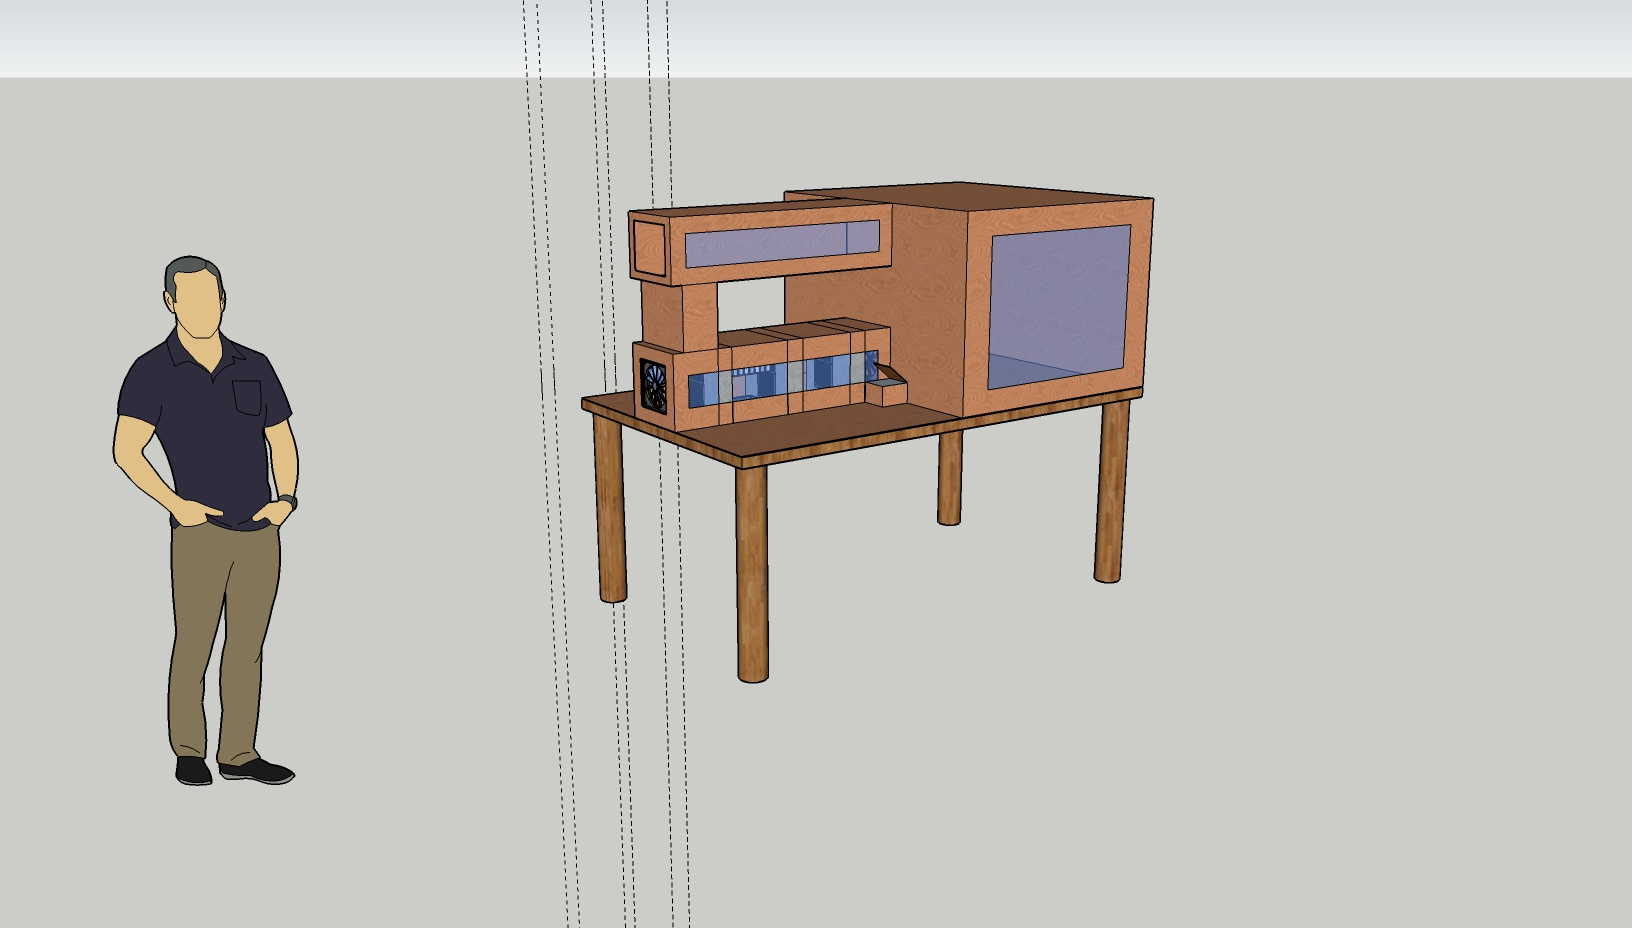
\includegraphics[width=\textwidth]{images/titlepic.jpg}}

\maketitle

\chapter*{Summary}
\addcontentsline{toc}{chapter}{Summary}
Air handling units are complex machines. To help students understand them
better, they need hands-on experience with a unit. However, real units are too
large and too expensive for most schools, and simulations are not accurate
enough. Therefore, we were tasked with designing, creating and programming a
miniature prototype of an air handling unit. This unit had several requirements
concerning temperature, humidity, and \ce{CO2} sensors, and actuators for air
speed, heating, cooling, and humidity.

We built a wooden case, we decided on a Raspberry Pi \cite{RaspberryPi}
(hereafter often referred to as simply ``Raspberry'' or ``Pi'') as the
controller, and wrote an API in \Cpp to communicate with the sensors and
actuators. We are controlling the heating and cooling elements, the fans, and
the servos for the vents using PWM. The temperature and humidity sensors are
controlled using I2C, and communication with the \ce{CO2} sensors occurs using
UART.

To operate the air handling unit, and to create some example code, we built a
control application with a web interface. This application can manually control
the actuators and reads out all of the sensors. In the end, most of the
requirements were successfully fulfilled.


\chapter*{Introduction}
\addcontentsline{toc}{chapter}{Introduction}
Air handling units are complex machines with a lot of variables, all of which
can have an influence on the way the system works. This makes it difficult for
students to fully comprehend systems like these so that they are able to design
and implement air handling units themselves. The problem with normal sized air
handling units is that they are just too big. How can students experiment with
it to get an understanding of how an air handling unit works? Currently, the
only possible way is with simulators. But as with every simulator, there is the
question if they are realistic enough. Are they applicable for students who
want to learn how an air handling unit works? The answer is no. While they
perform the basic functions, there are ways to make a room even hotter than the
sun. This is of course not physically possible. That's why we were given the
task to create a scaled down model of a normal sized air handling unit.
Designing, building and coding the system to be working at the demonstration
all need to be done within this assignment. 

Designing the build was the first thing addressed during the project. During
this stage research had to be done on what components would be used, which type
of material to use and all the measurements had to be calculated. The decision
of what parts or components to use was also based on the given requirements.
The research on the components can be found in the "Hardware" sections of this
report, and the requirements are available in Chapter \ref{ch:requirements}.

Building the unit itself was done after research was finished. This task
contained getting the resources, cutting them to the calculated measurements
and assembling everything. More in-depth information on this subject can be
found in Section \ref{sec:case} -- Case.

At last the code had to be written for all the components. In the beginning all
the components were tested separately of each other. This meant coding went per
component. After coding all the components, everything was put together to make
an complete API which we decided to complement with a control software to
demonstrate the API in action. Information about this subject can be found in
Chapter \ref{ch:software} - Software.

\setcounter{tocdepth}{1}
\tableofcontents
\mainmatter
\chapter{Approach}
In the beginning of the project, we decided on using Scrum \cite{scrum}. Scrum
is a project methodology that would allow us to quickly get a working
prototype, on which we could then apply improvements in fast iterations. It is
also a methodology we have used before, which means we could get started
quickly without having to learn new procedures.

Our plan was to take the first three weeks as "Sprint 0", to formulate a plan
of approach and get all requirements and plans figured out. This plan of
approach can be found in Appendix \ref{app:plan-of-approach}, a short outline
or our planning is given here.

In the next sprint (sprint 1), we were going to start our research, and we were
going to design our prototype. We were also going to start building the
prototype. In sprint 2, the plan was to have finished our research. We also
wanted to our prototype hardware complete. In this second sprint, we were also
planning on starting on software development for the prototype. The plan then
was to have a working prototype in sprint 3, at the assessment of the first
half of the project.

In sprints 4 through 7 (weeks 4.1 - 4.8), our plan was to elaborate the control
program in two-week iterations. In the meantime, we were going to evaluate the
hardware and improve it if necessary.


\chapter{Requirements}
\label{ch:requirements}
In order to design the air handling unit and to make sure the choices made are
in line with the desires of the client, clear requirements need to be defined.
These requirements can be split into two types: functional requirements,
defining the functions that the air handling unit must or should be able to
carry out, and non-functional requirements, defining certain preconditions that
the design should be compliant with.

\section{Functional requirements}
In essence, the function of an air handling unit is fairly simple, which is why
there are not a lot of functional requirements. The air handling unit must be
able to measure \ce{CO2} levels, humidity levels, and temperature. It must also
be able to control those levels, using a variety of actuators. It should also
be possible for users of the unit to readout the measured levels, and determine
how the air handling unit responds to those measurements in order to control
the actuators.

In the first meeting with the client, he indicated he wanted a chamber size of
approximately \SI{50x50x50}{\cm}. He also expressed the wish that the
specifications of the mock-up unit should be similar to those of real air
handling units. The desired chamber size leads to a volume of \SI{125}{\L}.
During our excursion to Systemair %TODO
, we discovered that an air handling unit is
supposed to refresh all of the air in the building three times per hour.
Plugging in those numbers leads to an airflow of \SI{375}{\L\per\hour}, or
\SI{104.2}{\cm\cubed\per\s}. To simulate an air handling unit in Dutch weather,
we looked at data from the KNMI (Royal Dutch Weather Institute), which showed
the lowest average minimum temperature in February is \SI{-1.0}{\celsius}
\cite{knmi-min-feb}, and the highest average maximum temperature in August is
\SI{24.0}{\celsius} \cite{knmi-max-aug}. To take some margins into account, we
assumed an intake air temperature between \SI{-10}{\celsius} and
\SI{30}{\celsius} four our calculations. We also assumed a desired room
temperature between \SI{18}{\celsius} and \SI{25}{\celsius}.  The relative
humidity should ideally be between 50\% and 60\%, but anywhere between 30\% and
70\% is acceptable.  The relative humidity of the intake air (assuming the
Dutch climate) can be anywhere between 20\% and 100\% \cite{knmi-relh}.  The
temperature and relative humidity are within these ranges in many parts of the
world, so designing the air handling unit according to these criteria should
mean it can be used by students worldwide.

\section{Non-functional requirements}
Because of the specific purpose of this mock-up air handling unit, there are
many more non-functional requirements, which are in some cases more important
than the functional requirements in making certain decisions. First, the air
handling unit must be built out of materials that are easily available to any
technical educational institution anywhere in the world, so that anyone needing
to instruct students on the workings of an air handling unit can build a
mock-up similar to ours. This also means the cost of the materials needs to as
low as possible. Building the air handling unit should also be very simple.

\chapter{Components}

\section{Controller}
\subsection{Hardware}
For the controller, we considered five options: a Raspberry Pi
\cite{RaspberryPi}, a single-board PC from a different manufacturer
\cite{BananaPi}, an Arduino \cite{Arduino}, a microcontroller chip with our own
circuits around them \cite{AtMega}, or a fully fletched desktop. Each of these
options had their own advantages and disadvantages. A Raspberry Pi has the
advantages of being widely available and easily programmable. It also easily
supports a screen, and has built-in support for the protocols of the available
sensors. It also has WiFi and Bluetooth on board. The disadvantages are that
the input/output ports function at \SI{3.3}{\volt}, and have a very limited
power delivery.

The single-board PC from a different manufacturer is very similar to the
Raspberry Pi, except that it can deliver more power. However, it is twice as
expensive as the Raspberry Pi, and it is less well known, which means that it
isn't as widely available and has less of a support community.

The Arduino has the advantages of being a highly adaptable, low-power board,
which functions completely at \SI{5}{\volt} logic levels. It also has a lot of
input/output pins, and is widely available worldwide. The disadvantages are
that it requires a computer to program it, and that loading programs onto the
Arduino can be a little complicated and prone to errors. It is also not
possible to connect anything but a very simple LED display to an Arduino.

A microcontroller in a home-made circuit is in essence very similar to an
Arduino, except that it is a lot cheaper. This price difference comes with a
tradeoff, namely that it requires a lot of time and effort to develop the
circuit. The home-made circuit also makes the system harder to reproduce than
when using any other controller.

The last option we looked into was a fully fletched desktop computer. The price
of such a system can vary a lot, but it is more expensive than any of the other
choices. The advantages are that a desktop computer is powerful,
multifunctional and easily programmable. The disadvantages are that a desktop
computer does not have any real input/output ports, which makes it a lot harder
to interact with sensors and actuators, and that it is too expensive.

After weighing all the advantages and disadvantages, we decided that using a
Raspberry will be the best option for this project, because of the easy
reproducibility, the relatively low  costs, and the easily accessible
input/output ports. As a added bonus we can display a monitoring UI on the
supported hdmi interface which shows a real time representation of the unit

The controller unit is installed to the right of the intake tube of the air
handling unit. Next to the two breadboards which is where all the cables from
the sensors and actuator are combined and eventually are connected to the
Raspberry Pi. The setup for the demo is using a consumer wireless solution to
create a local network for the Raspberry Pi and developers PCs. The router is
setup with a static DHCP lease for the Raspberry Pi MAC address for easy
connection even when we switch to a different setup. Power is delivered through
a standard 2 Amp Micro-USB wall adapter. This could however be changed too feed
directly from the power supply but for the demo setup is was preferred to
separate the two so that in the case of an overload or other incident we could
turn off the power supply without shutting down the Raspberry Pi.

\begin{figure}[h]
\centering
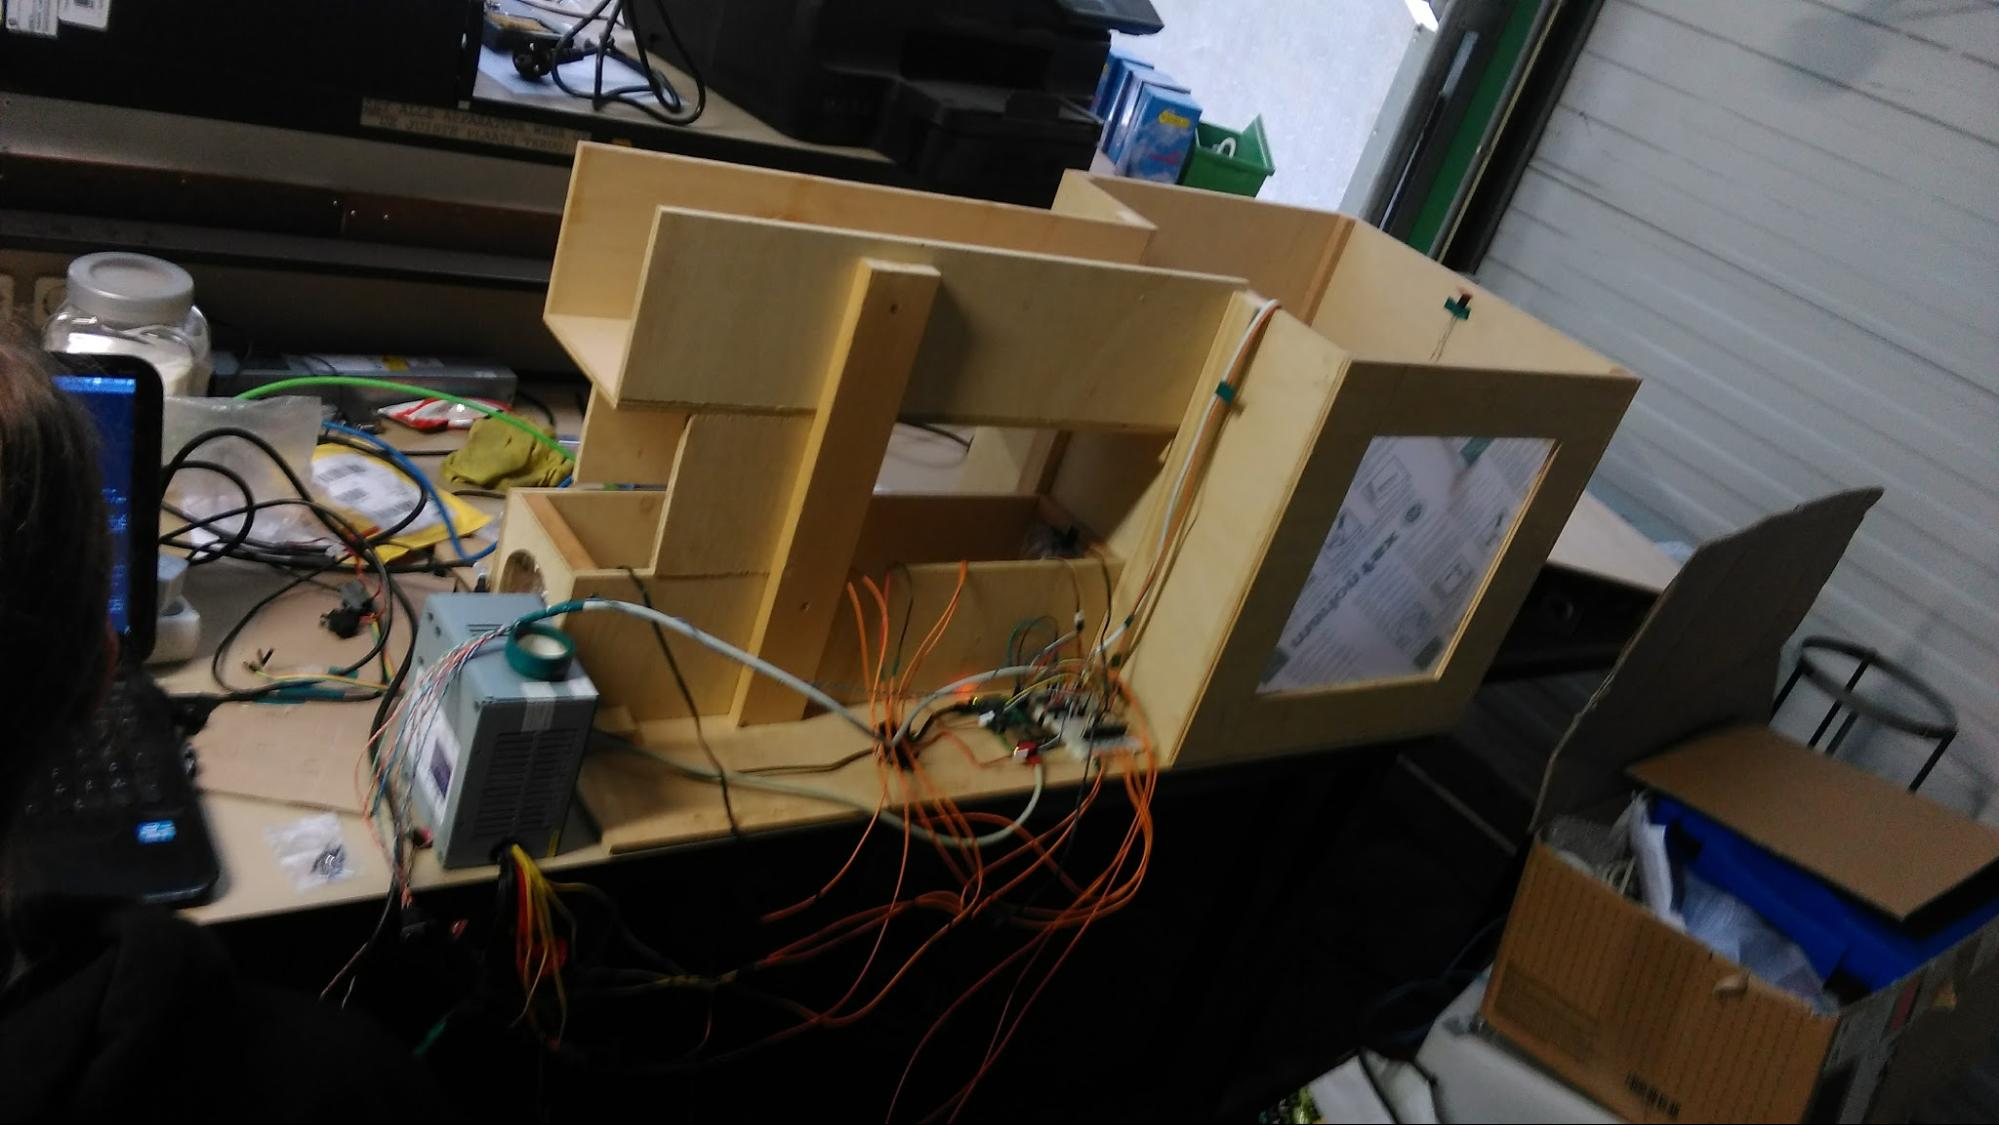
\includegraphics[width=0.8\textwidth]{images/casebuilt.jpg}
\caption{A picture of the case in-progress, with the Raspberry Pi installed.}
\label{fig:case}
\end{figure}

\subsection{Software}
The Raspberry Pi is running Raspbian Jessie Lite\footnote{Raspbian
\cite{Raspbian} is the official supported operating system for the Raspberry
Pi, based on the Debian Linux distribution \cite{Debian}. Jessie is the
previous version of Raspbian, the most recent version (``Stretch'') was
released in the summer of 2017. The ``Lite'' version does not include a desktop
environment.} which due to being a Linux distribution is easy to administer
over an SSH connection from one of the development PCs. Code is imported to
the Pi via Git\footnote{Git is a distributed version control system, originally
created for the development of the Linux kernel \cite{Git}}. If one of the
developers pushes a new version it is pulled to the Pi and compiled through a
custom makefile which first compiles the API (if necessary) to object files.
Next, it compiles the main controller program, and finally it links all object
files together into a single executable.

\subsection{Problems}
While setting up the Raspberry Pi we encountered a couple problems. During our
first setup of Raspbian we used a cheap poor quality SD card which resulted in
agonisingly slow install and update times. This was however resolved when we
received the 16GB Class 10 SD card. Class 10 means the card has a minimal
sequential writing speed of 10MB/s, as well as having a higher reading speed
than the cheap SD card we used earlier. The other problem we ran into was with
the ip address since we did not install a monitor and we did not have any way
to check what ip address got assigned by the router. We fixed this by using our
own router with a static DHCP binding.

\subsection{Recommendations}
We would recommend using a high quality SD card class 10 or similar. We also
recommend implementing a way to power the Raspberry Pi from the power supply,
while keeping it separate from the rest of the components, to be able to shut
down the components without powering off the Raspberry Pi.

\section{Case}
\label{sec:case}
\subsection{Hardware}
For the building materials the choice came down to three choices: metal, wood
and plastic. 

\begin{table}[]
\centering
\makebox[\textwidth][c]{
\begin{tabular}{llll}
              & \textbf{Metal}                      & \textbf{Wood} & \textbf{Plastic}         \\ \hline
Advantages    & Very sturdy                         & Not affected by temperature   & Lightweight              \\
              & Strong while thin                   & Easy to shape                 & Cheap                    \\
              & Medium availability                 & Cheap                         & Relatively easy to shape \\
              &                                     & Easy to mount together        &                          \\
              &                                     & Easy to replace a small piece &                          \\
              &                                     & High availability             &                          \\ \hline
Disadvantages & Affected by temperature             & Affected by water             & Hard to mount together   \\
              & Hard to shape                       & Not as sturdy as metal        & Affected by temperature  \\
              & Chance of electrical short-circuits &                               & Low availability         \\
              & As TI hard to weld together         &                               &                         
\end{tabular}
}
\caption{Comparison of materials}
\label{tab:materials}
\end{table}

With the considerations, given in Table \ref{tab:materials}, we went for wood.
Wood is the easiest to adjust and has a high availability, so later on it will
be easy for other students to replicate it, as stated in the non-functional
requirements. Of course it's possible to create the mock-up with metal or
plastic, but for our timespan, skills and the assignment requirements wood was
the best choice.

While buying the wood plate and while holding it we concluded that the
\SI{4}{\mm} plate would not be enough for the case. So we decided to go with a
double thickness and bought a \SI{9}{\mm} thick plywood plate. We first started
cutting the one \SI{244x122}{\cm} hardwood plywood plate in sections as
outlined in our design. After that we cut out a piece of \SI{35x35}{\cm}
perspex for the window. Then we started to assembly of the case this took
considerable amount of time. During this time we decided to go with modular
setup so that we could easily change the wiring and install additional
compartment walls. After completing the main chamber and fixing some off the
measuring flaws, we needed to cut of some edges which were forgotten to be
taken into account, we started on the first tube. This intake tube will be
housing for all of the actuators and most of the sensors. Due to this fact we
made the top of this part slidable so we could reach in and place/replace
components. The same is true for tunnel connecting it to the upper tube. Too
support this tube and since there is no complete interconnect we installed some
support beams to support the upper tube. We then finished the case by
installing the upper tube.

\subsection{Problems}
We ran into a amount of problems the first being was easily fixed but worth
noting. While buying the stock wood plate we had the plate cut at the store but
due to a mistake from the store clerk we ended up with wrong size pieces.
After some complaining with the store we got replacement parts so we ended up
with extra pieces. This ended up helping later with our next problem while we
were building the case we ended up missing a couple mm on either side of the
tube walls this was due to the original design being meant for \SI{4}{\mm}
thick wood but we went with \SI{9}{\mm} because we found that \SI{4}{\mm} would
not be structurally sound enough. Another problem we ran into while
constructing the case was because a \SI{9}{\mm} sheet is still rather thin the
nails would split the plywood to fix this we used small wood strips this also
helped with the modular approach we went with because now we could support the
top piece of the tubes on the strips without nailing them too the rest of the
case.

\subsection{Recommendations}
We would recommend that future prototypes use even thicker material or use
better support strips this would also allow for almost complete use of screws
instead of nails this would make taking the case apart for changes easier as
well as making the case more rigid and stronger overall. If you would use
materials that are more than \SI{2}{\cm} thick you could even forgo the use of
support material what would give the case a more aesthetically pleasing look
and more place for cables and components. Also to complete the case when all
the components are installed we would recommend using silicon sealant to make
the case airtight and to make the whole case airtight we recommend using a
rubber ring and a pressure locking mechanisms to seal the top of the main
chamber. Another recommendation would be to implement an efficient cable
management route instead of bent over nails.

\section{Heating elements}
\subsection{Hardware}
To calculate the power requirements of the heating elements, we will assume the
worst-case scenario, whereby the intake temperature is \SI{-10}{\celsius}, and
the desired temperature of the air in the chamber is \SI{25}{\celsius}. Using a Mollier
diagram (see Figure \ref{fig:mollier}), we can figure out how much energy this needs. The
vertical axis is the temperature of the air in \si{\celsius}, the horizontal axis is the
absolute humidity in kg water per kg air. The curved lines are lines of equal
relative humidity, while the diagonal lines are the amount of energy in a kg of
air, relative to the chosen origin of \SI{0}{\celsius} without any humidity.

Heating up air means moving straight up in the diagram, because the temperature
changes without affecting the absolute humidity. This means if we heat the air
up from \SI{-10}{\celsius} to \SI{25}{\celsius} at zero humidity, we need to go
from \SI{-10}{\J\per\kg} to \SI{25}{\J\per\kg}, adding \SI{35}{\J\per\kg}. If
we start at 100\% humidity, we start at \SI{-6}{\J\per\kg} and go to
\SI{29}{\J\per\kg}, so we are also adding \SI{35}{\J\per\kg}. In Chapter
\ref{ch:requirements}, we calculated that the air needs to be flowing at
\SI{104.2}{\cm\cubed\per\s}. The density of air is \SI{1.225}{\kg\per\m\cubed},
so we will need to heat up about \SI{1.28e-4}{\kg\per\s}, which (plugging in
the \SI{35}{\J\per\kg}) requires approximately \SI{0.00447}{\J\per\s}, or about
\SI{4.47}{\milli\W}. However, if we use the airflow as described in Section
\ref{sec:fans} of \SI{140.3}{\m\cubed\per\hour}, we get
\SI{38,972}{\cm\cubed\per\s}, or \SI{0.0477}{\kg\per\s}, which means we need
about \SI{1.67}{\W}. However, this power requirement does not contain any power
needed to compensate for the cooling element. As visible in Section
\ref{sec:cooling}, the cooling element will cool the air no more than
\SI{25}{\celsius}, which means the calculated \SI{1.67}{\W} is at least half of
the total power required. This means that (factoring in some margins) a total
heating power of at least \SI{5}{\W} should be enough for our purposes. Because
our design uses two heating elements, the required power rating of each heating
element is \SI{2.5}{\W}.

\begin{figure}[h]
\centering
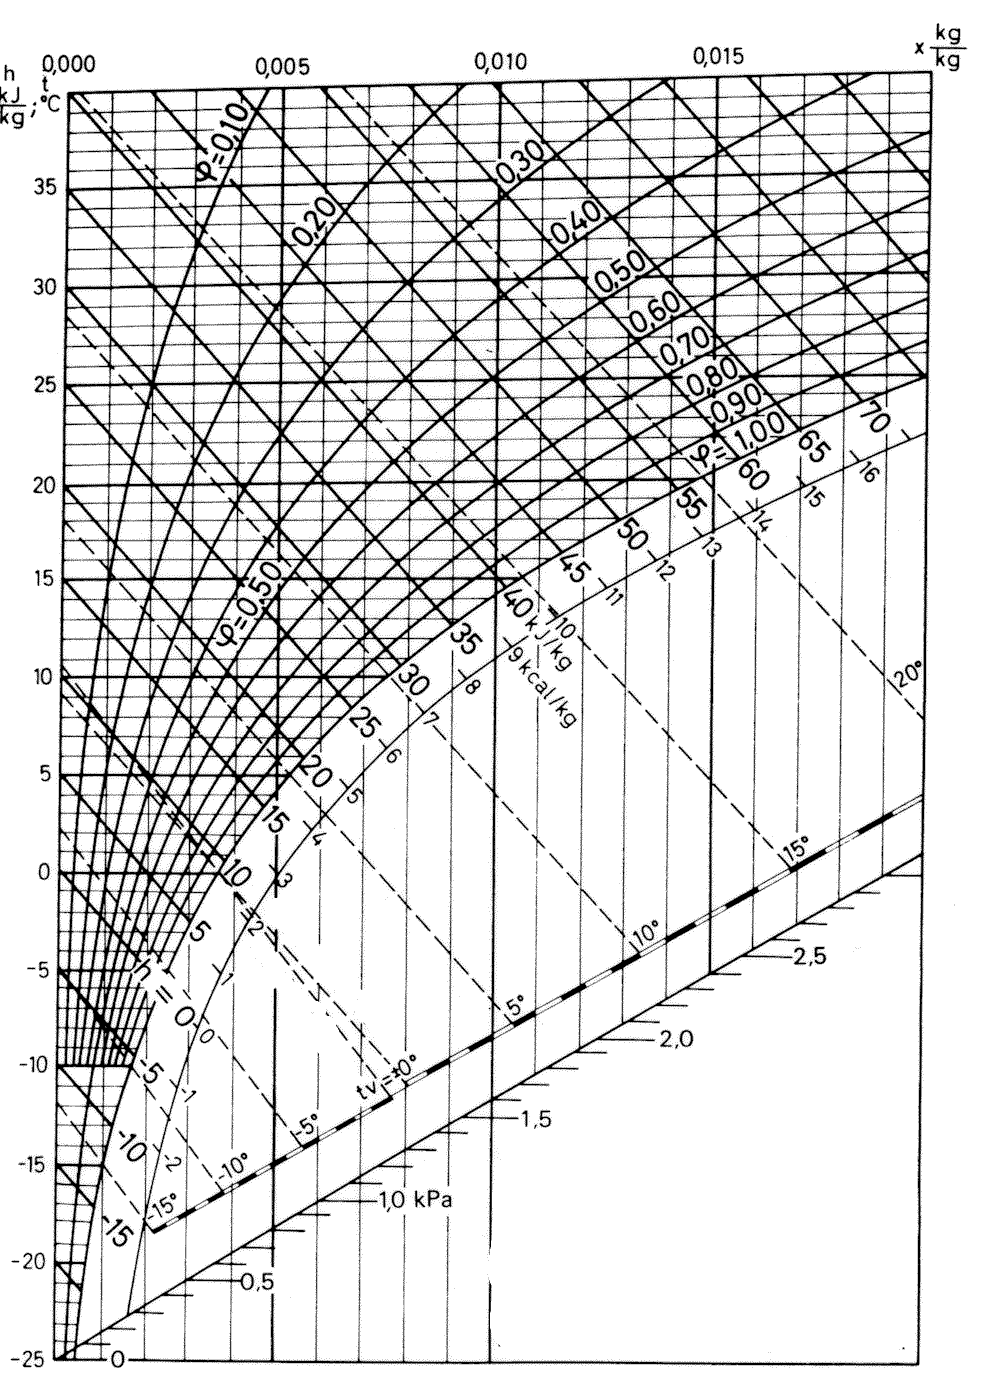
\includegraphics[width=0.8\textwidth]{images/mollier.png}
\caption{Mollier diagram. \protect\cite{mollier}}
\label{fig:mollier}
\end{figure}

For the heating elements, we had a choice out of several possibilities. In
regular-sized air handling units, air is heated using hot water, which usually
comes from a gas-burning heater. However, due to the complexity of a design
using hot water, we had been given the task of finding a purely electrical
heater. Electrical heating elements are practically all based on a resistance
wire, which heats up if a current flows through it. The differences between the
elements come from the length and width of the wire (which determine voltage
and power requirements), and from the type of the element the wire is embedded
in. For the type of the element, we found three widely available options: a
tube-shaped element with slats, a ceramic element, or a resistance wire without
an element around it. Each of these options has its own advantages and
disadvantages.

The tube-shaped element as visible in Figure \ref{fig:tube-heating} is
specially designed to heat air, and it's a standard element that's easy to
connect. The disadvantages are that tube-shaped elements are all rated at 230V,
which means we will need a powerful relais switch. There also isn't a wide
range of power available. A last and critical disadvantage is that the shortest
tube-shaped elements have a minimum length of \SI{200}{\mm}, while for our
design the maximum length of the heating element is \SI{150}{mm}. This means
there is no way to fit a tube-shaped element into the air handling unit.

\begin{figure}[h]
\centering
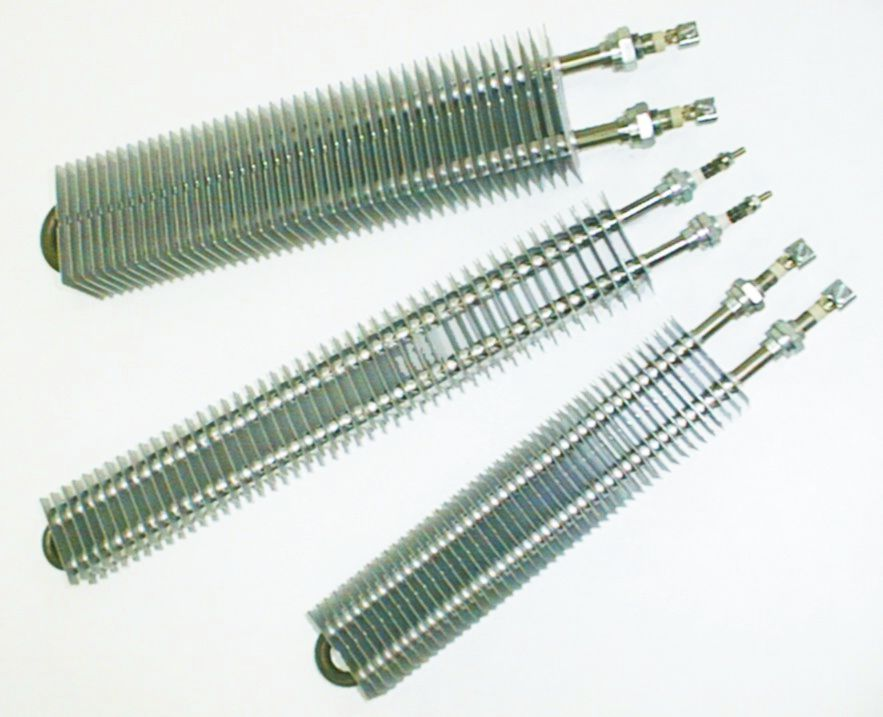
\includegraphics[width=0.8\textwidth]{images/tube-heater.jpg}
\caption{Tube-shaped heating elements. \protect\cite{tube-heater}}
\label{fig:tube-heating}
\end{figure}

The ceramic elements have several advantages: they are available in a wide
variety of sizes and shapes, have a large range of possible power ratings, and
are available both in \SI{230}{\V} and \SI{12}{\V} versions. The main
disadvantage is that the only ceramic element available at Conrad, pictured in
Figure \ref{fig:ceramic-heating}, is smaller than we would like it to be. This
element is \SI{90x27x17}{\mm}, which means we will have to figure out a way to
prevent the air from flowing around it instead of through the element.

\begin{figure}[h]
\centering
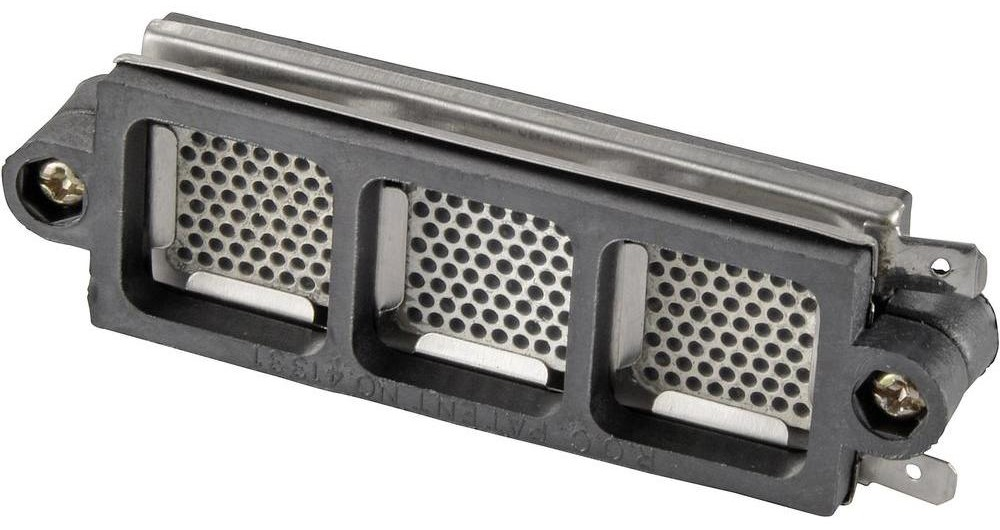
\includegraphics[width=0.8\textwidth]{images/ceramic-heater.jpg}
\caption{Tube-shaped heating elements. \protect\cite{ceramic-heater}}
\label{fig:ceramic-heating}
\end{figure}

Lastly, there is the option to purchase a spool of resistance wire, as pictured
in Figure \ref{fig:wire-heating}. The advantage is that we can choose the length of the
resistance wire, which means any combination of power, voltage and amperage is
possible. However, this advantage does not weigh up against the disadvantages:
if we use a resistance wire, we have to build a system to transfer the energy
efficiently to the air, while at the same time preventing short circuits or
electric shocks. There is also a chance that the resistance wire gets very hot
in certain places, which has a non-negligible risk of fire.

\begin{figure}[h]
\centering
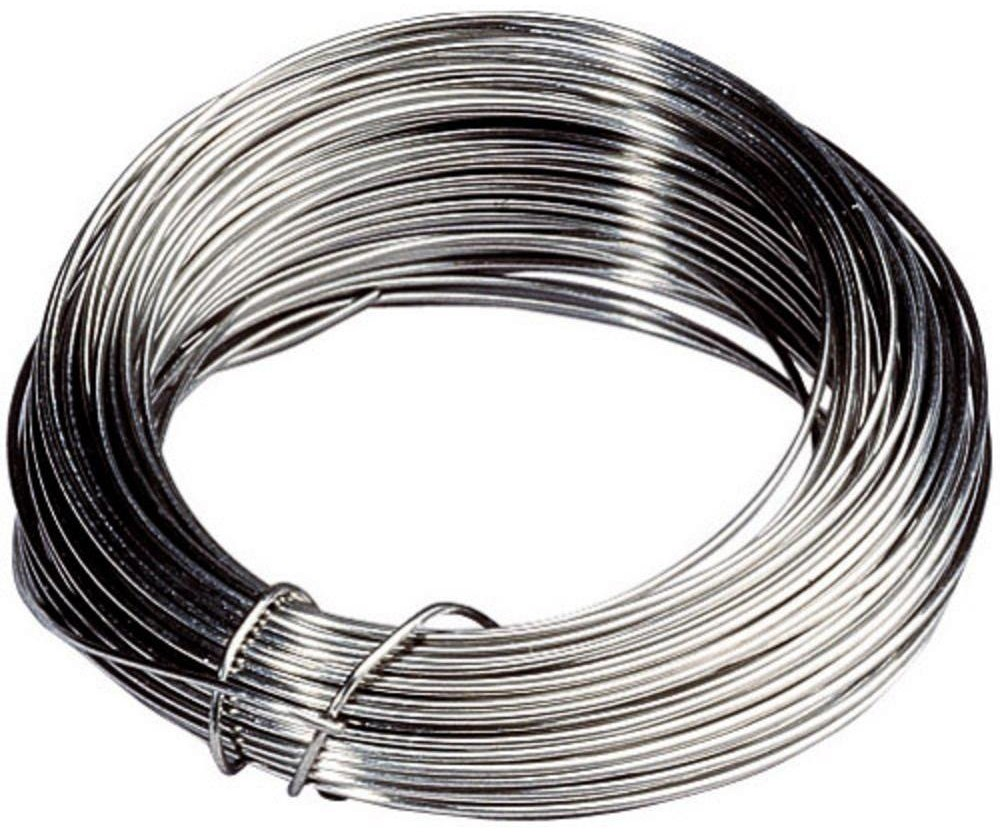
\includegraphics[width=0.8\textwidth]{images/wire-heater.jpg}
\caption{Tube-shaped heating elements. \protect\cite{wire-heater}}
\label{fig:wire-heating}
\end{figure}

In conclusion, we decided that a resistance wire would be too difficult to
implement safely, because of the risks of electric shocks or fire. It also
would not fit with the idea of an air handling unit mock-up that is easily
built by others. The choice was now between the tube-shaped element or the
ceramic element. Because of the tube-shaped elements are only available
starting at \SI{200}{\mm}, we decided on using a ceramic element, because it
fits better in our design. The only ceramic heating element that would not have
to be shipped overseas (thus requiring too long of a delivery time) was the
small \SI{150}{\W} element mentioned earlier. This element can deliver more
power than we need, but this mainly means it will not have to be switched on
continuously.

This element when it was received tested and we observed that it heats up
incredibly fast. However we were using simple underpowered transistors, which
heated up and failed very fast. During this time we decided to wire up the
heating elements and place them in the case and order mosfets that would be
able to withstand the immense current required for the heating elements.
However, these have not been delivered yet and could not be installed for this
reason.

\subsection{Software}
To accurately control the heating elements, we are using a PWM signal to
rapidly turn a transistor on and off. To do this, we created the PWM class,
which we will explain first. This class implements the iCommunication
interface, so it has the standard \lstinline|Initialize()|, \lstinline|Read()|
and \lstinline|Write()| functions (lines 6, 8, 9). The \lstinline|Read()|
function is empty on purpose, because it is not possible to read from a PWM
pin. Due to the specifics of the softPwm API of the WiringPi library, we need a
more sophisticated Initialize function which receives a list of pins that will
be used for PWM signals.  Therefore, the standard \lstinline|Initialize()|
function will always return false.

\lstinputlisting{code/pwm-class.h}

The \lstinline|Initialize()| function receives an array of GPIO pins that will
be used for PWM signals. All of these are initialized with the
\lstinline|softPwmCreate()| function.  This function also requires an initial
value and a maximum value. In our case, we always set the initial value to 0 to
make sure the pin is turned off. The maximum value is always set to 100, which
means we can set the pin to anywhere between 0 and 100.

\lstinputlisting{code/pwm-initialize.cpp}

The \lstinline|Write()| function only requires a data value and an address. All
it does is call the \lstinline|softPwmWrite| function. Since this function has
no error checking, we can not detect whether or not the call has succeeded.

\lstinputlisting{code/pwm-write.cpp}

The heating element class, HeatingElement, is relatively simple, and inherits
from the iActuator class. Its most important function is
\lstinline|SetValue()|. This function first limits the value to within an
acceptable range, and then calls the \lstinline|SetValue()| function of the
parent class. The acceptable range for the heating elements is between 0 and
30, because that ensures the transistors do not get too hot.

\lstinputlisting{code/heating-setvalue.cpp}

The \lstinline|SetValue()| function of the iActuator class is very simple. All
it does is call the \lstinline|Write()| function of the Communication member.

\lstinputlisting{code/iactuator-setvalue.cpp}

\subsection{Problems}
As alluded to in the hardware sections of the heating element the problem we
ran into with the heating element was not the heating element but rather the
hardware required to control the power of the element. We used TIP120
transistors but these are only rated for \SI{5}{\ampere} \cite{Transistor}
Since our heating elements each pull more than \SI{5}{\ampere} \cite{Heating}
the transistor heated up and melted. After this we did not use the transistors
to control the heating element anymore and tested the api software using a
voltmeter. 

\subsection{Recommendations}
We would recommend using a mosfet like FQP30N06L. These are rated for up to
\SI{32}{\ampere} \cite{FQP30N06L}, this will be more than enough to handle the
heating elements. However this only covers a very simple use case and to safely
and efficiently implement this we would recommend someone with the required
knowledge of electronics  to design an analog circuit which can handle the high
frequency pwm without potentially breaking the power supply and maybe even
separate the elements completely from the Raspberry Pi.   

\section{Cooling element}
\label{sec:cooling}

\subsection{Hardware}
The cooling element in a regular air handling unit is based on
vapor-compression, but due to the size of this solution it is not applicable on
this small-scale model. As a replacement of the vapor-compression based cooling
element we choose to go with a Peltier-element, which cools based on
thermoelectric cooling. The pros for us are the size, prize and the fact there
are no moving parts. The cooling element is not only used to reduce the
temperature of the room it is aswell used to reduce the humidity in the air and
that is where the cooling potential of the element comes in.If we take the
worst case scenario of 100\% humidity to 20\% humidity as stated in the
requirements we need to cool the air down from \SI{25}{\celsius} to
\SI{5}{\celsius}. So we need atleast a temperature difference of maximum
outside temperature as in the requirements specified minus \SI{5}{\celsius} for
the humidity to get to the minimum humidity. This results in a total
\SI{25}{\celsius} temperature difference.

\begin{table}[]
\centering
\makebox[\textwidth][c]{
\begin{tabular}{l|ll}
Category               & Hightech Peltier element & Hightech Peltier element \\ \hline
Type                   & QC-127-1.4-8.5MD         & QC-241-1.0-3.9M          \\
Rated Voltage          & \SI{15.5}{\V}            & \SI{29.5}{\V}            \\
Max. current           & \SI{8.5}{\A}             & \SI{3.9}{\A}             \\
Wattage (max.)         & \SI{72}{\W}              & \SI{64}{\W}              \\
Temperature difference & \SI{71}{\K}              & \SI{71}{\K}              \\
Sizes                  & \SI{40x40x3.4}{\mm}      & \SI{40x40x3.6}{\mm}      \\
Price                  & \euro 43,54              & \euro 61,01                 
\end{tabular}
}
\caption{Comparison of materials}
\label{tab:peltier}
\end{table}

Table \ref{tab:peltier} shows a variety of Peltier elements. We chose to go
with the lower voltage one to be compliant with the power requirements of other
components. Both of the elements are in the range of the temperature difference
specified in the above part.

Our chamber is pretty small so we don't need a huge cooling surface, but we
wanted to place a cooling element on the cold side of the element to help with
the disperse of the cold. This heatsink however has not been installed yet both
due to not having been bought. Also during the testing of the element we found
out that because the device transfers heat from one of its sides too the other
there will have to be another heatsink with fan to dissipate the heat. These
however also haven't been bought yet and so have not been installed yet. Wiring
has been done but due to the fact the heat can't be dissipated right now we
can't run the element for long periods of time.

\subsection{Software}
The code for the cooling element is completely identical to that of the heating
elements. It also uses the PWM class, and its \lstinline|SetValue()| function
also limits the value to the 0-30 range before calling the parent class
\lstinline|SetValue()| function.

\subsection{Problems}
We ran into two problems with our cooling element, the first being the same as
with the heating element. The cooling element also draws too much power which
overloads the transistor. The other problem was that in order to function the
element needs to dissipate the heat it extracts from the cold side on the hot
side. But since we did not know this during our design phase this wasn't
included in the design. To compensate for this we needed to cut a hole in the
top of the lit of the intake tube. This would give space to install a heatsink
and maybe a fan. But again due to this item not being able to be bought in time
this hasn't been installed yet.

\subsection{Recommendations}
The same recommendation as for the heating element stands, we recommend using a
mosfet that supports the amperage required for the cooling element.
Additionally we recommend looking into other methods of cooling because while
this approach will work but the heat will be dissipated in close vicinity of
the intake which may interfere with the process.

\section{Temperature and humidity sensors}
\subsection{Hardware}
When researching the temperature and humidity sensors, our original plan was to
have separate temperature sensors and humidity sensors. However, it turned out
that almost all humidity sensors can also report the temperature, so in the end
we decided to use combined temperature/humidity sensors. For the sake of
completeness, our original research into temperature-only sensors is also
described here.

\subsubsection{Temperature-only sensors}
Beginning the research process, all components were researched separate of each
other. That's why the temperature sensors were also researched as
temperature-only sensors. While there are hundreds of sensors that read the
temperature, within this research there were a couple of options. Each option
doing the same thing but with different maximum temperature readings,
connection types or just costs. One however stood out because of the way it
communicated with a controller. It was the DS18B20. The way this sensor
communicates with the controller is by a 1-wire interface and an unique
identifier. This meant that there could be multiple sensors connected to a
single interface on the controller where every sensor is reached by its
identifier. As the ports on the controller were limited for the project's
needs, this was the sensor of choice. This sensor also met all the other
requirements. For example, it can read temperatures from \SI{-55}{\celsius} to
\SI{+125}{\celsius}. This was more than enough looking at the functional
requirements in Chapter \ref{ch:requirements}, where it is stated that we will
be measuring temperatures from \SI{-10}{\celsius} to \SI{+30}{\celsius}.
However since there are sensors where the temperature and humidity sensors are
combined, it was decided that buying one sensor with two operations is the way
to go. Another reason for going with this decision was because of the physical
layout, the temperature sensor would sit next to a humidity sensor at all
times.

\subsubsection{Combined temperature and humidity sensors}
Early on in the design process, we decided on using I2C to communicate with the
humidity sensors, because it allows many devices to be placed on a single bus.
However, when researching the humidity sensors, it turned out there are many
humidity sensors that only have a single fixed I2C address. There were a few
with the possibility to select one of two I2C addresses, and we found one
sensor that allows a choice between four different I2C addresses.

As visible in Table \ref{tab:humidity}, this was the Texas Instruments HDC1010
\cite{HDC1010}. Using the HDC1010, we'd have to use two I2C busses. While there
is a second I2C bus on the Raspberry Pi, enabling it is not straightforward and
requires both changing kernel configuration files and soldering a header onto
the Raspberry Pi. Another disadvantage of the HDC1010 is that it's only sold as
a surface-mount device, which means it needs to be soldered onto a PCB by
baking it. While there exist breakout boards for the HDC1010, they were all out
of stock or discontinued.

Another option was to use an I2C multiplexer, and a simple humidity sensor with
one I2C address. We found several of these, their details are listed in Table
\ref{tab:humidity}. It becomes apparent that there is a fairly direct
relationship between price and capabilities. The more you pay, the higher range
and the better accuracy you get. Because all three sensors are good enough for
our purposes, we chose to use the Silicon Labs Si7021 \cite{Si7021}, the
cheapest of the three.

For the I2C multiplexer, the one that was recommended to us online was the
Texas Instruments TCA9548A \cite{TCA9548A}, which is an easily controllable
multiplexer. It is readily available on a breakout board from several Dutch
online stores, and does not cost much.

\begin{table}[]
\centering
%\makebox[\textwidth][c]{
\begin{tabular}{lllll}
Name                 & HDC1010                & HTU21D                 & Si7021                & SHT31-D                \\ \hline
No. of I2C addresses & 4                      & 1                      & 1                     & 1                      \\
Min. temp            & \SI{5}{\celsius}       & \SI{-40}{\celsius}     & \SI{-10}{\celsius}    & \SI{-40}{\celsius}     \\
Max. temp            & \SI{60}{\celsius}      & \SI{125}{\celsius}     & \SI{85}{\celsius}     & \SI{125}{\celsius}     \\
Temp. uncertainty    & \SI{\pm0.2}{\celsius}  & \SI{\pm0.3}{\celsius}  & \SI{\pm0.4}{\celsius} & \SI{\pm0.3}{\celsius}  \\
Min. humidity        & \SI{0}{\percent}       & \SI{5}{\percent}       & \SI{0}{\percent}      & \SI{0}{\percent}       \\
Max. humidity        & \SI{100}{\percent}     & \SI{95}{\percent}      & \SI{80}{\percent}     & \SI{100}{\percent}     \\
Humidity uncertainty & \SI{\pm2}{\percent}    & \SI{\pm2}{\percent}    & \SI{\pm3}{\percent}   & \SI{\pm2}{\percent}    \\
Price                & \euro 2,52             & \$14.95                & \$6.95                & \$13.95
\end{tabular}
%}
\caption{Comparison of temperature and humidity sensors \protect\cite{HDC1010}
\protect\cite{HTU21D} \protect\cite{Si7021} \protect\cite{SHT31-D}}
\label{tab:humidity}
\end{table}

When we chose to go with the combined sensor which includes both the humidity
and the temperature sensors, we chose to go with Si7021. These I2C-enabled
sensor have hardcoded I2C addresses, in this case as shown in the datasheet
0x40 \cite{Si7021}. To overcome this problem we installed an I2C multiplexer, a
TCA9548A. This multiplexer is where all of the wiring harnesses are connected.
After wiring the wiring harnesses which include power, ground and sda/scl for
each individual sensor, we routed them through the case. The wires are capped
off at each end with headers so we can easily swap out components if they
break. The power for the sensors is supplied by the power supply, and is routed
through the breadboard to the sensors. This was needed because the Raspberry Pi
was not capable of delivering the required power. 

\subsection{Software}
\subsubsection{Sensors}
The the temperature and humidity sensors are very similar in code, because they
both read data from the Si7021 chips. They both implement the iSensor abstract
class, and the only differences are in the \lstinline|GetValue()| function.

The \lstinline|Humidity::GetValue()| function first calls the \lstinline|Communication->Write()|
function (line 4), with the data byte 0xF5. This data byte is the command for
"Measure relative humidity" \cite{Si7021}. After that, the
relative humidity can be fetched with a call to \lstinline|Communication->Read()| (line 8).
Next, we convert the two bytes received into an integer, and use that to
calculate the relative humidity in percent using the formula in \S5.1.1 of the
Si7021 Datasheet (lines 10-11).

\lstinputlisting{code/humidity-getvalue.cpp}

The temperature is measured in a very similar manner. There are two
differences: we write byte 0xE0 ("Read Temperature Value from Previous RH
Measurement") instead of 0xF5, and the formula for calculating the temperature
is \lstinline|double temperature = (175.72*result) / 65536 - 46.85| (Si7021
Datasheet, \S5.1.2)

\subsubsection{Multiplexer}
Because all the Si7021 chips use the same I2C address, they can not be
connected to the same I2C bus. This is why we decided to use an I2C
multiplexer. All of the code to handle the multiplexer is in the I2C class.

First, the I2C class implements the iCommunication interface. This means it has
a \lstinline|Write()| function, which writes a byte to an address, and a \lstinline|Read()| function,
which reads data into a buffer. It also has some helper functions, namely
\lstinline|_setSlave()|, \lstinline|_write()|, and \lstinline|_writeByte()|.

\lstinputlisting{code/i2c-class.h}

To fully understand the I2C class, let's walk through a call to
\lstinline|Write()|. The \lstinline|Write()| function takes two parameters: the
byte to send (\lstinline|data|), and the address, which is a number from 1 to
8, depending on which pins of the multiplexer we want to use. First, we check
if the multiplexer is already set to the address we need to talk to (line 2).
If it is, we immediately go to the \lstinline|_write()| call at the end of the
function (line 8). If it is not, we first call \lstinline|_setSlave()| (line
3).

\lstinputlisting{code/i2c-write.cpp}

\lstinline|_setSlave()| first creates a bitmask for the multiplexer to work
with (line 2) (source: TCA9548A datasheet). Next, it calls \lstinline|_write()|
to write the bitmask to the multiplexer (line 3). If the \lstinline|_write()|
call succeeds, we also save the \lstinline|currentTarget| (line 4).

\lstinputlisting{code/i2c-_setslave.cpp}

The \lstinline|_write()| function uses the syscall \lstinline|ioctl()| (line
2), which tells Linux which slave address to use for the next I2C read and
write calls (source: Kernel i2c documentation). (N.B.: the filedescriptor is an
integer which points to the \lstinline|/dev/i2c-1| special file. This file is
opened in the constructor.) Next, it calls \lstinline|_writeByte()| to actually
send the data to the I2C bus (line 8).

\lstinputlisting{code/i2c-_write.cpp}

Last, there is the \lstinline|_writeByte()| function. This function first
creates a two-character buffer, containing the data byte and a null character
(line 2).  Next. we call the syscall \lstinline|write()|, which requires a
null-terminated character array (line 4). If the syscall succeeds, we have
succesfully written the data byte to the I2C bus.

\lstinputlisting{code/i2c-_writebyte.cpp}

Completely separate from the write functions, there is the
\lstinline|I2C::Read()| function. First, we create a temporary buffer to store
data in (line 2). Next, we keep trying to read data into this buffer from the
I2C special file (line 5). Once we succeed, we copy all but the last byte
(which is the end-of-file marker) from the temporary buffer to the buffer that
was provided by the caller (line 14).

\lstinputlisting{code/i2c-read.cpp}

\subsection{Problems}
One of the problems we could have run into was that of addressing the Si7021
sensors, because their I2C address is not modifiable. Thankfully, we foresaw
this issue, so we dealt with it by purchasing an I2C multiplexer. Another issue
is that in the current design of the code, after a measurement command, the
program blocks while the measurement is being taken. This means the system
could noticeably slow down if this part of the API is used in larger systems
with more sensors. It currently is not a problem because the system does not
have to be fast. Finally the Raspberry Pi wasn't capable of delivering the
required amount of power; this was resolved by powering them from the power
supply directly.

\subsection{Recommendations}
We would recommend using sensors with programmable addresses because this would
greatly simplify the cable harness and eliminate the need for a multiplexer.

\section{\ce{CO2} sensors}
\subsection{Hardware}
The \ce{CO2} sensors are needed to measure how much fresh air the unit needs to
take in to control the \ce{CO2} level in the room.  There are several options
to measure the \ce{CO2}, one of which is the NDIR-type sensor. NDIR stands for
non-dispersive infrared, which is a principle to detect the existence of
\ce{CO2} in the air. The benefit of an NDIR sensor is that an NDIR sensor
already has a built-in heating element, which is necessary for measuring the
\ce{CO2} levels. If we go for a non-NDIR sensor, we also have to provide an
external heating source to measure the \ce{CO2} level. By choosing an NDIR
sensor we don't need an extra heating element, therefore the controls of the
\ce{CO2} sensor are simpler than with a non-NDIR sensor where you have to
control the sensor and the external heating element. This makes it easier for
the students who are going to work with the air handling unit to get a general
overview of the unit, without having to delve into the details of the \ce{CO2}
sensor. It also makes it easier for them to change the sensor for another model
if they have little programming skills. That's why we chose an NDIR-type
\ce{CO2} sensor.

For our purposes, mentioned earlier,  we decided to use an MH series \ce{CO2}
sensor. The MH series has small sensor who could fit easily in the unit and
they are relatively cheap for an NDIR \ce{CO2} sensor. Therefore the choice
came down to two sensors, the MH-Z14a and the MH-Z19, which are compared in
Table \ref{tab:co2}.

\begin{table}[]
\centering
\makebox[\textwidth][c]{
\begin{tabular}{l|ll}
                    & MH-Z14a                                    & MH-Z19                      \\ \hline
Working voltage     & \SIrange{4.5}{5.5}{\volt}                  & \SIrange{4.5}{5.5}{\volt}   \\
Average current     & \SI{<60}{\milli\A}                         & \SI{<85}{\milli\A}          \\
Interface Level     & \SI{3.3}{\volt} (\SI{5}{\volt} compatible) & \SI{3.3}{\volt}             \\
Measuring range     & \SIrange{0}{10000}{ppm}                    & \SIrange{0}{5000}{ppm}      \\
Output signal       & PWM                                        & PWM                         \\
                    & UART                                       & UART                        \\
					& Analog voltage signal                      & Analog voltage signal       \\
Preheat time        & 3 min                                      & 3 min                       \\
Working temperature & \SIrange{0}{50}{\celsius}                  & \SIrange{0}{50}{\celsius}   \\
Working humidity    & \SIrange{0}{90}{\percent RH}               & \SIrange{0}{90}{\percent RH}\\
Dimension (LxWxH)   & \SI{57.5x34.7x14.6}{\mm}                   & \SI{57.5x34.7x16}{\mm}
\end{tabular}
}
\caption{Comparison of \ce{CO2} sensors \protect\cite{mh-z14a} \protect\cite{mh-z19}}
\label{tab:co2}
\end{table}

The working temperatures of both sensors don't go as far as the
\SI{-10}{\celsius} described
in the function requirements, but this applies to all the sensors in our price
range. If we go for a \ce{CO2} sensor that is capable of working in
\SI{-10}{\celsius} and has a
good availability, the price would be about ten times higher as the price is
now. For that reason we went for a sensor with a working temperature that only
goes to \SI{0}{\celsius}, but is affordable and fits inside the budget.

The MH-Z14a has a measuring range from 0 to 10000 ppm (parts per million).
Legally the maximum allowed \ce{CO2} value is 1000 ppm in the Netherlands
\cite{bouwbesluit}. Knowing this, the measuring range of the MH-Z19, which is 0
to 5000 ppm, will be more than enough. Furthermore, it is going to be difficult
to reach a \ce{CO2} value higher than 5000 ppm in our mock-up.

Therefore the choice went to the MH-Z19 NDIR sensor, as depicted in Figure
\ref{fig:mh-z19}. The functionality is as good as the MH-Z14a, while the
MH-Z19 is a bit cheaper, fits better in our design and has a better
availability.

\begin{figure}[h]
\centering
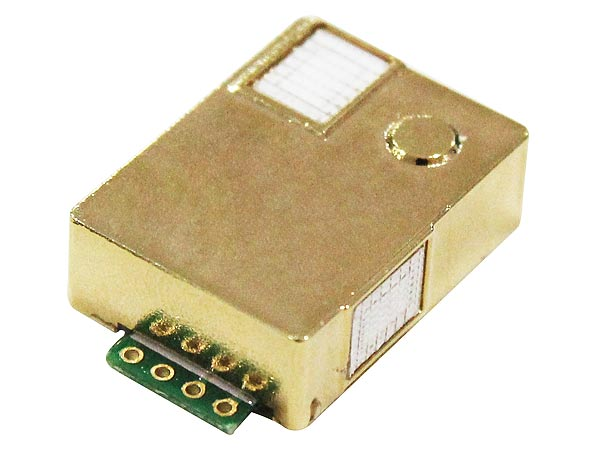
\includegraphics[width=0.8\textwidth]{images/co2.jpg}
\caption{MH-Z19 \ce{CO2} sensor \protect\cite{mh-z19}}
\label{fig:mh-z19}
\end{figure}

We decided to use the UART communication capabilities of the MH-Z19. This
immediately presented a problem as the Raspberry Pi only has one UART
interface, and since the sensor address is hardwired in the sensor, we needed
to find a solution. By wiring the transmit pin to both sensors and the receive
wires to different pins on the Raspberry Pi we could distinguish between the
two sensors. These wires were also incorporated into the cable harness but due
to them working on \SI{5}{\volt} instead of the \SI{3.3}{\volt} on which the
I2C works they needed a different power line. 

\subsection{Software}
The chosen hardware, MH-Z19, has 2 manners of sending data to the Raspberry Pi.
The first being a PWM signal and the second being UART. After researching the
possibilities we decided on working with UART. This way of communicating is in
this case only used for the \ce{CO2} sensors. 

\subsubsection{Serial}
To get serial communication working on a Raspberry Pi which is running Linux, a
few values need to be changed within the OS its files. These values keep the
serial port occupied for the OS itself, which in our case is not good as we
need that port to communicate. These values have to be changed by calling the
\lstinline|raspi-config| and disabling serial communication for the OS. Another
change has to be done in the file \lstinline|/boot/cmdline.txt| where the
specified port name is set to the OS it's communication, which in our case
again needs to be released.

After doing this the port is open to use and will work with any code. The
initialization for serial is seen below:

\lstinputlisting{code/serial-initialize.cpp}

Line 3 opens the serial port with line 4 to 7 being its error handling. Line 9
to 16 contain the settings that are used for the serial communication, for
example \lstinline|baudrate = 9600| and no parity.

Besides this the Serial class has two other functions, The \lstinline|Read()|
and \lstinline|Write()| functions. While the only main function for using
serial for the \ce{CO2} sensor is reading the value, you have to write to the sensor
to give it a signal to start a measurement.

The write function can be seen below:

\lstinputlisting{code/serial-write.cpp}

Line 6 to 15 define the array that is sent to the \ce{CO2} signal to trigger it to
start the measurement, this array is predefined by the makers of the MH-Z19 and
can be traced back to its datasheet \cite{mh-z19}. This is hardcoded within the
write function because this was just not taken into account. At the time of
coding the code was written with the array hardcoded for testing reasons and
speed up the process of getting everything working. Line 19 is where the data
is sent to the sensor with line 20 to 25 being its error handling.

The read code:

\lstinputlisting{code/serial-read.cpp}

The main code of this function is put in a while because the port needs to be
open for data reading. Whenever the data is read once, the while loop stops and
the function carries on. The main read of data is done on line 10, after which
the \ce{CO2} specific decoding is done and the global variables are set.

\subsubsection{Sensors}
The \ce{CO2} sensors have a specific class as well. This class is for the component
management and is used to handle the received data. As a class itself this
isn't the most complicated class because a part of the handling is done by the
serial class. 

The main function of the class, \lstinline|getValue()| can be seen below:

\lstinputlisting{code/co2-getvalue.cpp}

The function simply calls the \lstinline|Write()| function of the communication
class followed by a \lstinline|Read()| call. The value that comes out of this
is then recalculated to the exact format, ppm in this case and then returned to
be stored by the Controller class. The way the ppm has to be calculated is also
specified in the datasheet \cite{mh-z19}.

\subsection{Problems}
If using multiple CO2 sensors there is a problem. The ID's of the sensors can't
be changed so the identification of multiple sensors is difficult to do when
they are all connected to the same serial port. A solution for this problem is
using a multiplexer or using a different GPIO pin for each sensor, in which
case the sensors can be kept separate of each other. So the program writes to
all sensors at one time and reads on different GPIO pins

\subsection{Recommendations}
We would recommend using a multiplexer if it's desired to have even more
sensors, in other cases using different GPIO pins for each sensor will suffice.

\section{Fans}
\label{sec:fans}
\subsection{Hardware}
The fans are used to blow the air through the handling tunnel into the room.
There are two fans in our air handling unit, one to take air into the handling
tunnel and one at the end of the handling tunnel just before the air enters the
room. We placed the second fan so that the intake air doesn't go into the
tunnel for return air, but goes straight into the room. 

The kind of fan they use in a real air handling unit is way too powerful and
too big for our mock-up. In fact, almost all normal fans are too big for our
purpose. To solve this problem we came up with a computer fan, which are small
but still relatively powerful. 

The only important specification for the fan are the sizes and that the rpm
must be controllable, so that the intake of air can be controlled.

After some research, we came to the Aerocool Shark Fan, which is depicted in
Figure \ref{fig:fan}. With its \SI{12}{\cm} diameter it will fit into the
\SI{15x15}{\cm} handling tunnel. Because of its three pin connection it is
possible to control the rpm.  As stated in the functional requirements, the air
handling unit needs to be able to refresh the room at least three times per
hour. That came down to the fan needing to be capable of moving
\SI{104.2}{\cm\cubed} air per hour. As visible in Table \ref{tab:fan}, the
Aerocool Shark Fan has an maximum airflow of \SI{140.3}{\metre\cubed\per\hour},
which is more than enough to refresh the room three times per hour. The fan of
choice actually is a bit overpowered but the air we need to move to refresh the
room three times per hour is very low, which makes almost every computer fan
suitable for out mock-up, as long as the rpm is controllable. 

A last argument is that the fan is not that expensive and has a good
availability at several webshops.

\begin{table}[]
\centering
\makebox[\textwidth][c]{
\begin{tabular}{ll}
Power connection & 3-pin                             \\
Voltage range    & \SIrange{7}{12}{\volt}            \\
Maximum rpm      & 1500 rpm                          \\
Volume           & \SIrange{12.6}{26.5}{\decibel}    \\
Maximum airflow  & \SI{140.3}{\metre\cubed\per\hour} \\
Power            & \SI{3.6}{\watt}                    \\
sizes(WxHxD)     & \SI{120x120x25}{\mm}
\end{tabular}
}
\caption{Aerocool Shark Fan specifications \protect\cite{aerocool}}
\label{tab:fan}
\end{table}

\begin{figure}[h]
\centering
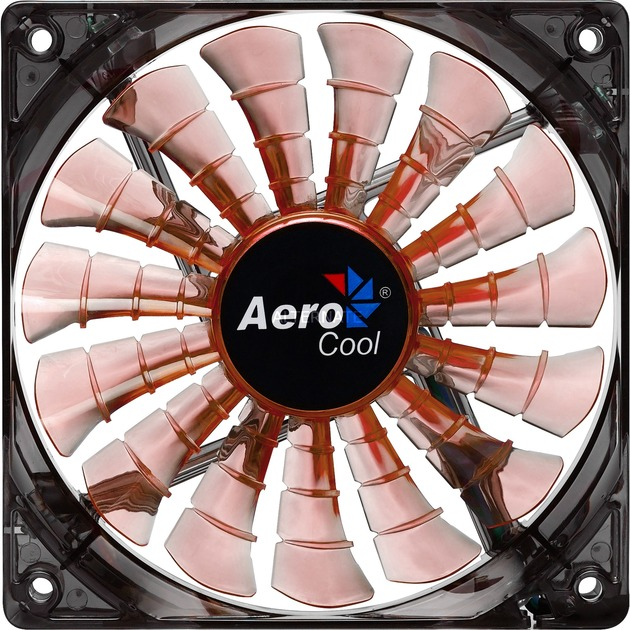
\includegraphics[width=0.8\textwidth]{images/fan.jpg}
\caption{Aerocool Shark Fan \protect\cite{aerocool}}
\label{fig:fan}
\end{figure}

However, due to ordering problems, we decided to use some cheap \SI{120}{\mm}
pc fans which we had laying around. The fans have been installed on either side
of the intake tube. These are connected to the power supply via two TIP120
transistors. While these were not powerful enough for the heating and cooling
elements, they are powerful enough for the fans.

\subsection{Software}
The code for the fans is very similar to that of the heating and cooling
elements. It also uses the PWM class to send a PWM signal, and it has a
\lstinline|SetValue()| function which limits the value to within an acceptable
range.  However, for the fans, we found that the acceptable range was between 0
and 100.

\lstinputlisting{code/fan-setvalue.cpp}

\subsection{Problems}
We didn't run into any problems with the fans. We however had some problems
with some wiring (we shorted a wire) but this was quickly discovered and fixed.

\subsection{Recommendations}

\section{Vents}
\subsection{Hardware}
\subsection{Software}
\subsection{Problems}
\subsection{Recommendations}

\section{Power supply}
\subsection{Hardware}
\subsection{Software}
\subsection{Problems}
\subsection{Recommendations}

\chapter{Software}
\label{ch:software}
\section{API}
\section{Control software}
\section{Webdesign}

\chapter{Conclusion}
\chapter{Evaluation and reflection}
\chapter{Bibliography}
\bibliographystyle{apacite}
\bibliography{bibliography.bib}

\appendix
\chapter{API Design}
\chapter{Control Software}
\chapter{Manual Control}
\chapter{Plan of Approach}
\label{app:plan-of-approach}
\chapter{API Code tutorial}
\chapter{Case tutorial}
\chapter{API Code documentation}

\end{document}
